\documentclass[11pt]{article}

%\usepackage{palatino}

\usepackage[utf8]{inputenc}
\usepackage[T1]{fontenc}
% Chivo como en las diapositivas o Fira Sans?
% \usepackage[familydefault,regular]{Chivo}
\usepackage[sfdefault,scaled=.85]{FiraSans}
\usepackage{newtxsf}
\usepackage[spanish]{babel}
\setlength{\parindent}{0pt}
\usepackage{amssymb}
\usepackage{amsmath}
\usepackage{wasysym}
\usepackage[x11names, rgb, html]{xcolor}
\usepackage{graphics}
\usepackage{caption}
\usepackage{lipsum}
\usepackage{float}
\usepackage{adjustbox}
\usepackage{geometry}
\usepackage[scaled=.85]{FiraMono}  

\geometry{left=3cm,right=3cm,top=3cm,bottom=3cm,headheight=1cm,headsep=0.5cm} 


%%% PGFPLOTSTABLE

\usepackage{pgfplotstable}

%%% COLORES


%% Colores de Solarized

\definecolor{sbase03}{HTML}{002B36}
\definecolor{sbase02}{HTML}{073642}
\definecolor{sbase01}{HTML}{586E75}
\definecolor{sbase00}{HTML}{657B83}
\definecolor{sbase0}{HTML}{839496}
\definecolor{sbase1}{HTML}{93A1A1}
\definecolor{sbase2}{HTML}{EEE8D5}
\definecolor{sbase3}{HTML}{FDF6E3}
\definecolor{syellow}{HTML}{B58900}
\definecolor{sorange}{HTML}{CB4B16}
\definecolor{sred}{HTML}{DC322F}
\definecolor{smagenta}{HTML}{D33682}
\definecolor{sviolet}{HTML}{6C71C4}
\definecolor{sblue}{HTML}{268BD2}
\definecolor{scyan}{HTML}{2AA198}
\definecolor{sgreen}{HTML}{859900}

%% Colores del documento

\definecolor{text}{RGB}{78,78,78}
\definecolor{accent}{RGB}{129, 26, 24}

%%% LISTINGS

\usepackage{listings}

%% Las tildes

\lstset{
  inputencoding=latin1
}

%% Colores de Solarized para listings

\lstset{
  % How/what to match
  % sensitive=true,
  language=C++,
  % Border (above and below)
  frame=lines,
  % Line number
  numbers=left,
  % Extra margin on line (align with paragraph)
  xleftmargin=\parindent,
  % Put extra space under caption
  belowcaptionskip=1\baselineskip,
  % Colors
  % backgroundcolor=\color{sbase3},
  basicstyle=\footnotesize\ttfamily\color{sbase00},
  keywordstyle=\color{scyan},
  commentstyle=\color{sbase1},
  stringstyle=\color{sblue},
  numberstyle=\color{sbase01},
  identifierstyle=\color{smagenta},
  % Break long lines into multiple lines?
  breaklines=true,
  % Show a character for spaces?
  showstringspaces=false,
  tabsize=2
}





\title{Algorítmica: práctica 2 \\ \large Mezclando $k$ vectores ordenados\\ \vspace{0.2em}Grupo 2}
\author{Sofía Almeida Bruno \and Antonio Coín Castro \and María Victoria Granados Pozo \and Miguel Lentisco Ballesteros \and José María Martín Luque}
\date{\today}

\begin{document}
\maketitle

\newpage

\section*{Introducción}

El objetivo de esta práctica es diseñar un algoritmo \textit{divide y vencerás}
que se encargue de combinar $k$ vectores ordenados. Además tenemos que analizar
su eficiencia, implementarlo y compararlo con un algoritmo clásico.

\section*{Algoritmo clásico}

\lstinputlisting[language=C++]{./../src/mezcla-vectores-clasicos.cpp}

\subsection*{Eficiencia teórica}

\subsection*{Eficiencia empírica}

\subsection*{Eficiencia \textit{híbrida}}

\section*{Algoritmo \textit{divide y vencerás}}

\subsection*{Eficiencia teórica}

\subsection*{Eficiencia empírica}

\subsection*{Eficiencia \textit{híbrida}}




\begin{center}
	% GNUPLOT: LaTeX picture with Postscript
\begingroup
  \makeatletter
  \providecommand\color[2][]{%
    \GenericError{(gnuplot) \space\space\space\@spaces}{%
      Package color not loaded in conjunction with
      terminal option `colourtext'%
    }{See the gnuplot documentation for explanation.%
    }{Either use 'blacktext' in gnuplot or load the package
      color.sty in LaTeX.}%
    \renewcommand\color[2][]{}%
  }%
  \providecommand\includegraphics[2][]{%
    \GenericError{(gnuplot) \space\space\space\@spaces}{%
      Package graphicx or graphics not loaded%
    }{See the gnuplot documentation for explanation.%
    }{The gnuplot epslatex terminal needs graphicx.sty or graphics.sty.}%
    \renewcommand\includegraphics[2][]{}%
  }%
  \providecommand\rotatebox[2]{#2}%
  \@ifundefined{ifGPcolor}{%
    \newif\ifGPcolor
    \GPcolortrue
  }{}%
  \@ifundefined{ifGPblacktext}{%
    \newif\ifGPblacktext
    \GPblacktextfalse
  }{}%
  % define a \g@addto@macro without @ in the name:
  \let\gplgaddtomacro\g@addto@macro
  % define empty templates for all commands taking text:
  \gdef\gplbacktext{}%
  \gdef\gplfronttext{}%
  \makeatother
  \ifGPblacktext
    % no textcolor at all
    \def\colorrgb#1{}%
    \def\colorgray#1{}%
  \else
    % gray or color?
    \ifGPcolor
      \def\colorrgb#1{\color[rgb]{#1}}%
      \def\colorgray#1{\color[gray]{#1}}%
      \expandafter\def\csname LTw\endcsname{\color{white}}%
      \expandafter\def\csname LTb\endcsname{\color{black}}%
      \expandafter\def\csname LTa\endcsname{\color{black}}%
      \expandafter\def\csname LT0\endcsname{\color[rgb]{1,0,0}}%
      \expandafter\def\csname LT1\endcsname{\color[rgb]{0,1,0}}%
      \expandafter\def\csname LT2\endcsname{\color[rgb]{0,0,1}}%
      \expandafter\def\csname LT3\endcsname{\color[rgb]{1,0,1}}%
      \expandafter\def\csname LT4\endcsname{\color[rgb]{0,1,1}}%
      \expandafter\def\csname LT5\endcsname{\color[rgb]{1,1,0}}%
      \expandafter\def\csname LT6\endcsname{\color[rgb]{0,0,0}}%
      \expandafter\def\csname LT7\endcsname{\color[rgb]{1,0.3,0}}%
      \expandafter\def\csname LT8\endcsname{\color[rgb]{0.5,0.5,0.5}}%
    \else
      % gray
      \def\colorrgb#1{\color{black}}%
      \def\colorgray#1{\color[gray]{#1}}%
      \expandafter\def\csname LTw\endcsname{\color{white}}%
      \expandafter\def\csname LTb\endcsname{\color{black}}%
      \expandafter\def\csname LTa\endcsname{\color{black}}%
      \expandafter\def\csname LT0\endcsname{\color{black}}%
      \expandafter\def\csname LT1\endcsname{\color{black}}%
      \expandafter\def\csname LT2\endcsname{\color{black}}%
      \expandafter\def\csname LT3\endcsname{\color{black}}%
      \expandafter\def\csname LT4\endcsname{\color{black}}%
      \expandafter\def\csname LT5\endcsname{\color{black}}%
      \expandafter\def\csname LT6\endcsname{\color{black}}%
      \expandafter\def\csname LT7\endcsname{\color{black}}%
      \expandafter\def\csname LT8\endcsname{\color{black}}%
    \fi
  \fi
    \setlength{\unitlength}{0.0500bp}%
    \ifx\gptboxheight\undefined%
      \newlength{\gptboxheight}%
      \newlength{\gptboxwidth}%
      \newsavebox{\gptboxtext}%
    \fi%
    \setlength{\fboxrule}{0.5pt}%
    \setlength{\fboxsep}{1pt}%
\begin{picture}(7200.00,4320.00)%
    \gplgaddtomacro\gplbacktext{%
      \colorrgb{0.30,0.30,0.30}%
      \put(1650,1060){\makebox(0,0)[r]{\strut{}$\textcolor{text}{1e-05}$}}%
      \colorrgb{0.30,0.30,0.30}%
      \put(1650,1580){\makebox(0,0)[r]{\strut{}$\textcolor{text}{0.0001}$}}%
      \colorrgb{0.30,0.30,0.30}%
      \put(1650,2100){\makebox(0,0)[r]{\strut{}$\textcolor{text}{0.001}$}}%
      \colorrgb{0.30,0.30,0.30}%
      \put(1650,2619){\makebox(0,0)[r]{\strut{}$\textcolor{text}{0.01}$}}%
      \colorrgb{0.30,0.30,0.30}%
      \put(1650,3139){\makebox(0,0)[r]{\strut{}$\textcolor{text}{0.1}$}}%
      \colorrgb{0.30,0.30,0.30}%
      \put(1650,3659){\makebox(0,0)[r]{\strut{}$\textcolor{text}{1}$}}%
      \colorrgb{0.30,0.30,0.30}%
      \put(1782,928){\rotatebox{45}{\makebox(0,0)[r]{\strut{}$\textcolor{text}{0}$}}}%
      \colorrgb{0.30,0.30,0.30}%
      \put(2093,928){\rotatebox{45}{\makebox(0,0)[r]{\strut{}$\textcolor{text}{500}$}}}%
      \colorrgb{0.30,0.30,0.30}%
      \put(2404,928){\rotatebox{45}{\makebox(0,0)[r]{\strut{}$\textcolor{text}{1000}$}}}%
      \colorrgb{0.30,0.30,0.30}%
      \put(2715,928){\rotatebox{45}{\makebox(0,0)[r]{\strut{}$\textcolor{text}{1500}$}}}%
      \colorrgb{0.30,0.30,0.30}%
      \put(3026,928){\rotatebox{45}{\makebox(0,0)[r]{\strut{}$\textcolor{text}{2000}$}}}%
      \colorrgb{0.30,0.30,0.30}%
      \put(3337,928){\rotatebox{45}{\makebox(0,0)[r]{\strut{}$\textcolor{text}{2500}$}}}%
      \colorrgb{0.30,0.30,0.30}%
      \put(3648,928){\rotatebox{45}{\makebox(0,0)[r]{\strut{}$\textcolor{text}{3000}$}}}%
      \colorrgb{0.30,0.30,0.30}%
      \put(3959,928){\rotatebox{45}{\makebox(0,0)[r]{\strut{}$\textcolor{text}{3500}$}}}%
      \colorrgb{0.30,0.30,0.30}%
      \put(4270,928){\rotatebox{45}{\makebox(0,0)[r]{\strut{}$\textcolor{text}{4000}$}}}%
      \colorrgb{0.30,0.30,0.30}%
      \put(4581,928){\rotatebox{45}{\makebox(0,0)[r]{\strut{}$\textcolor{text}{4500}$}}}%
      \colorrgb{0.30,0.30,0.30}%
      \put(4892,928){\rotatebox{45}{\makebox(0,0)[r]{\strut{}$\textcolor{text}{5000}$}}}%
    }%
    \gplgaddtomacro\gplfronttext{%
      \colorrgb{0.30,0.30,0.30}%
      \put(220,2359){\rotatebox{-270}{\makebox(0,0){\strut{}Tiempo de ejecución (s)}}}%
      \colorrgb{0.30,0.30,0.30}%
      \put(3337,220){\makebox(0,0){\strut{}Número de vectores (k)}}%
      \colorrgb{0.30,0.30,0.30}%
      \put(3337,3989){\makebox(0,0){\strut{}Algoritmos mezcla de k vectores}}%
      \csname LTb\endcsname%
      \put(6212,3549){\makebox(0,0)[r]{\strut{}Clásico}}%
      \csname LTb\endcsname%
      \put(6212,3329){\makebox(0,0)[r]{\strut{}DyV}}%
      \csname LTb\endcsname%
      \put(6212,3109){\makebox(0,0)[r]{\strut{}DyV STL}}%
    }%
    \gplbacktext
    \put(0,0){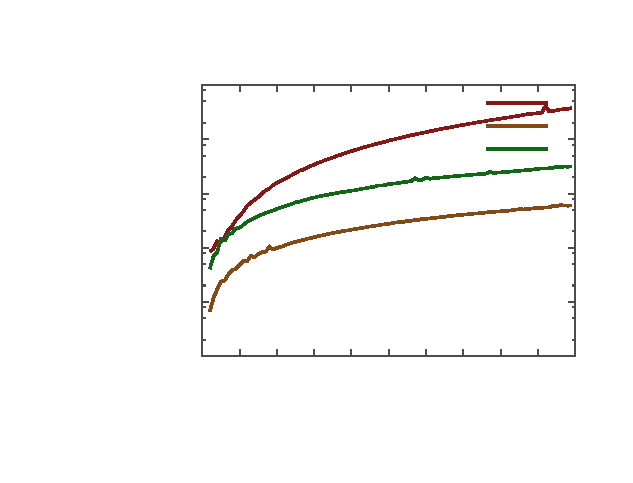
\includegraphics{./graficos/compare}}%
    \gplfronttext
  \end{picture}%
\endgroup

\end{center}













\section*{Algoritmos de ordenación}
\subsection*{Eficiencia $\boldsymbol{O(n^2)}$}
\subsubsection*{Burbuja}
Revisa cada elemento de la lista con el siguiente, intercambiándose de posición
si no están en el orden correcto. Su eficiencia teórica es $O(n^2)$.

\newpage
\subsubsection*{Inserción}
Consideramos el elemento N-ésimo de la lista y lo ordenamos respecto de los elementos desde el primero hasta el N-1-ésimo. Su eficiencia teórica es $O(n^2)$.

\subsubsection*{Selección}
Consiste en encontrar el menor de todos los elementos de la lista e intercambiarlo con el de la primera posición. Luego con el segundo, y así sucesivamente hasta ordenarlo todo. De nuevo, su eficiencia teórica es $O(n^2)$.


\subsection*{Eficiencia $\boldsymbol{O(n log n)}$}
\subsubsection*{Mergesort}
Se basa en la técnica de divide y vencerás. Consiste en dividir la lista en sublistas de la mitad de tamaño, ordenando cada una de ellas de forma recursiva. Si el tamaño de la lista es $0$ ó $1$ la lista ya está ordenada. Para acabar juntamos todas las sublistas en una sola. Su eficiencia teórica es $O(n\log n)$.


En este caso, podemos observar ciertas anomalías en la gráfica, pues presenta unos \textit{picos} para ciertos tamaños del vector. No sabemos bien a qué puede ser debido, pues hemos realizado cuidadosamente la ejecución en varias máquinas, así como en distintos sistemas operativos, obteniendo siempre el mismo resultado.

\subsubsection*{Quicksort}
También se basa en la técnica de divide y vencerás.
En primer lugar elegimos un elemento de la lista, que llamaremos \textit{pivote}. A continuación los elementos de la lista se ordenarán de forma que la derecha del pivote queden los mayores que él, y a la izquierda los menores. De esta forma dividimos la lista en dos sublistas, la de la derecha y la de la izquierda. Repetiremos el proceso mientras las sublistas tengan más de un elemento. Su eficiencia teórica también es $O(n\log n)$.


\subsubsection*{Heapsort}
Este algoritmo consiste en almacenar todos los elementos del vector a ordenar en una estructura de datos llamada montículo (\textit{heap}). Luego, se extrae el nodo que queda como nodo raíz del montículo (cima) en sucesivas iteraciones obteniendo el conjunto ordenado. Basa su funcionamiento en una propiedad de los montículos, por la cual, la cima contiene siempre el menor elemento (o el mayor, según se haya definido el montículo) de todos los almacenados en él. Su eficiencia teórica es $O(n\log n)$.\\

\newpage
\enlargethispage{7\baselineskip}
\section*{Otros algoritmos}
\subsection*{Floyd}
Es un algoritmo de análisis sobre grafos para encontrar el camino mínimo en grafos ponderados. El algoritmo compara todos los posibles caminos a través del grafo entre cada par de vértices. Es un ejemplo de \textbf{programación dinámica}, y su eficiencia teórica es $O(n^3)$.

\subsection*{Hanoi}
Hay tres pilas de discos, llamadas origen, auxiliar y destino. La primera de ellas está ordenada según tamaño creciente de los discos, de arriba hacia abajo. Se moverá un disco de la pila origen a la destino si hay un único disco en la pila origen. En caso contrario, se moverán todos los discos a la auxiliar, excepto el más grande. Por último, moveremos el disco mayor al destino, y movemos los $n-1$ restantes encima del mayor. El número de pasos crece exponencialmente con el número de discos, y su eficiencia teórica es $O(2^n)$.

\newpage
\section*{Cálculo de la eficiencia empírica}

Puesto que la eficiencia teórica de cada algoritmo es diferente, no podemos realizar las mediciones para los mismos valores de entrada en todos los algoritmos. Así, los agrupamos según su orden de eficiencia.\\

Para el cálculo de la eficiencia empírica, hemos utilizado un \textit{script} que realiza tantas ejecuciones de cada algoritmo como le indiquemos, tomando como parámetros el valor inicial, el incremento, y el valor final de los datos de entrada.\\

Las gráficas anteriores han sido realizadas a partir de los datos recogidos en las siguientes tablas.

\subsection*{Tablas}


\newpage
\subsection*{Gráficos comparativos}

A continuación se muestra una serie de gráficos que corresponden a la comparación de aquellos algoritmos que son de un mismo orden.

\subsubsection*{Algoritmos que son $\boldsymbol{O(n^2}$)}

\vspace{1em}
Observamos que el algoritmo \textbf{burbuja} es claramente más lento para estos valores. Esto se verá reflejado cuando calculemos los valores de las constantes ocultas en la eficiencia híbrida.


\subsubsection*{Algoritmos que son $\boldsymbol{O(n\log n}$)}

\vspace{1em}

Estos algoritmos se ejecutan en tiempos similares, aunque \textbf{quicksort} es ligeramente más rápido, manteniendo de forma uniforme la diferencia con los otros dos algoritmos a medida que aumenta el número de valores.

\subsubsection*{Algoritmos de ordenación}

\vspace{1em}

En este último gráfico, puede observarse claramente la tendencia de los algoritmos cuyo orden de eficiencia es $O(n\log n)$ a ser más rápidos que aquellos que son $O(n^2)$. Se ha utilizado una escala logarítmica para poder representar todos los algoritmos en un mismo gráfico.

\newpage


\section*{Cálculo de la eficiencia híbrida}
A continuación se recogen los gráficos que muestran tanto la eficiencia empírica como la función ajustada o \textit{eficiencia híbrida} de cada algoritmo. Para el ajuste, se ha utilizado la función que corresponde en cada caso a la eficiencia teórica de cada algoritmo. Además, utilizamos el mayor número de constantes ocultas posibles, a fin de que el ajuste sea mejor.\\

El valor de estas constantes ocultas puede verse reflejado también en las gráficas. Son precisamente estas constantes las que hacen que un algoritmo se ejecute más rápidamente que otro, aunque tengan el mismo orden de eficiencia teórica. 



\subsection*{Eficiencia $\boldsymbol{O(n^2)}$}

Para ajustar los algoritmos de ordenación cuadráticos hemos usado una función $f(x)$ de la forma: $$f(x) = a_0x^2 + a_1x + a_2$$ Con ayuda de \verb|gnuplot| hemos calculado los valores de las constantes ocultas, así como la gráfica que muestra tanto el ajuste como los valores experimentales.


\newpage
\subsection*{Eficiencia $\boldsymbol{O(n log n)}$}

La función utilizada para ajustar los valores en los algoritmos de ordenación de orden superlineal es: $$f(x) = a_0xlog(x) + a1x + a2$$


\subsection*{Eficiencia $\boldsymbol{O(n^3)}$}

En el caso del algoritmo de Floyd la función $f(x)$ utilizada es: $$f(x) = a_0x^3 + a_1x^2 + a_2x + a_3$$.


\subsection*{Eficiencia $\boldsymbol{O(2^n)}$}

Por último, ajustamos el algoritmo de Hanoi mediante la función: $$f(x) = a_02^{a_{1}x + a_2}$$ obteniendo el resultado mostrado a continuación.


En general, las constantes ocultas tienen un valor muy pequeño, en algunos casos del orden de $10^{-9}$. Esto es porque el ordenador ejecuta los algoritmos en cuestión de segundos o milésimas de segundo, para los tamaños de entrada relativamente “pequeños” que hemos introducido.

\newpage

\section*{Comparativa según optimización y sistema operativo}
Hemos elegido un representante de cada orden de eficiencia, y hemos realizados una comprativa para analizar cómo varían los tiempos de ejecución según el sistema operativo y el nivel de optimización.\\

Para cada algoritmo seleccionado veremos dos gráficas: una que compara la ejecución sin optimización en los sistemas operativos \textit{macOS} y \textit{Linux}; y otra que compara la ejecución en \textit{Linux} con los distintos tipos de optimización del compilador.

\subsection*{Representante de $\boldsymbol{O(n^2)}$ : Inserción}


\subsection*{Representante de $\boldsymbol{O(n\log n)}$ : Quicksort}

\subsection*{Representante de $\boldsymbol{O(n^3)}$ : Floyd}


\subsection*{Representante de $\boldsymbol{O(2^n)}$ : Hanoi}



Podemos observar en los cuatro casos que las variaciones entre ejecuciones en distintos sistemas operativos es prácticamente inapreciable, salvo alguna excepción. Del mismo modo, los tiempos de ejecución disminuyen significativamente, en general, de manera proporcional al nivel de optimización, tal y como cabía esperar.

\newpage

\section*{Ajuste con otras funciones}

Veamos por último lo que ocurre si intentamos ajustar los datos recogidos experimentalmente a una función que no coincide con la eficiencia teórica del algoritmo.


\fontsize{11pt}{7.2}\selectfont
Observamos que la curva ajustada y los datos experimentales no coinciden apenas que en unos cuantos puntos. Esto era de esperar, pues hemos ajustado los datos con funciones que difieren notablemente de su eficiencia teórica.

\newpage

\section*{Anexo}
\subsection*{Características de los ordenadores donde se ha ejecutado}

\vspace{0.5em}

\begin{enumerate}
\item Apple MacBook Pro, Intel(R) Core(TM) i5-5257U CPU @ 2.70GHz, 8GB RAM.\\  Compilador: clang-800.0.38 \\
  Sistema operativo: macOS Sierra
\item Dell XPS 13, Intel(R) Core(TM) i5-7200U CPU @ 2.50GHz, 8GB RAM.\\
  Compilador: g++ 6.3.1\\
  Sistema operativo: Arch Linux
\end{enumerate}


\end{document}

